% \Image{Capa do livro (; )}{PNLD2022-018-01.png}

% \Image{Ilustração do livro (; )}{PNLD2022-018-04.png}
% \Image{Ilustração do livro (; )}{PNLD2022-018-05.png}
% \Image{Ilustração do livro (; )}{PNLD2022-018-06.png}


\documentclass[11pt]{extarticle}
\usepackage{manualdoprofessor}
\usepackage{fichatecnica}
\usepackage{lipsum,media9}
\usepackage[justification=raggedright]{caption}
\usepackage[one]{bncc}
\usepackage[lunna]{../edlab}
\usepackage{marginnote}
\usepackage{pdfpages}
\usepackage[printwatermark]{xwatermark}
%\newwatermark[pagex=2]{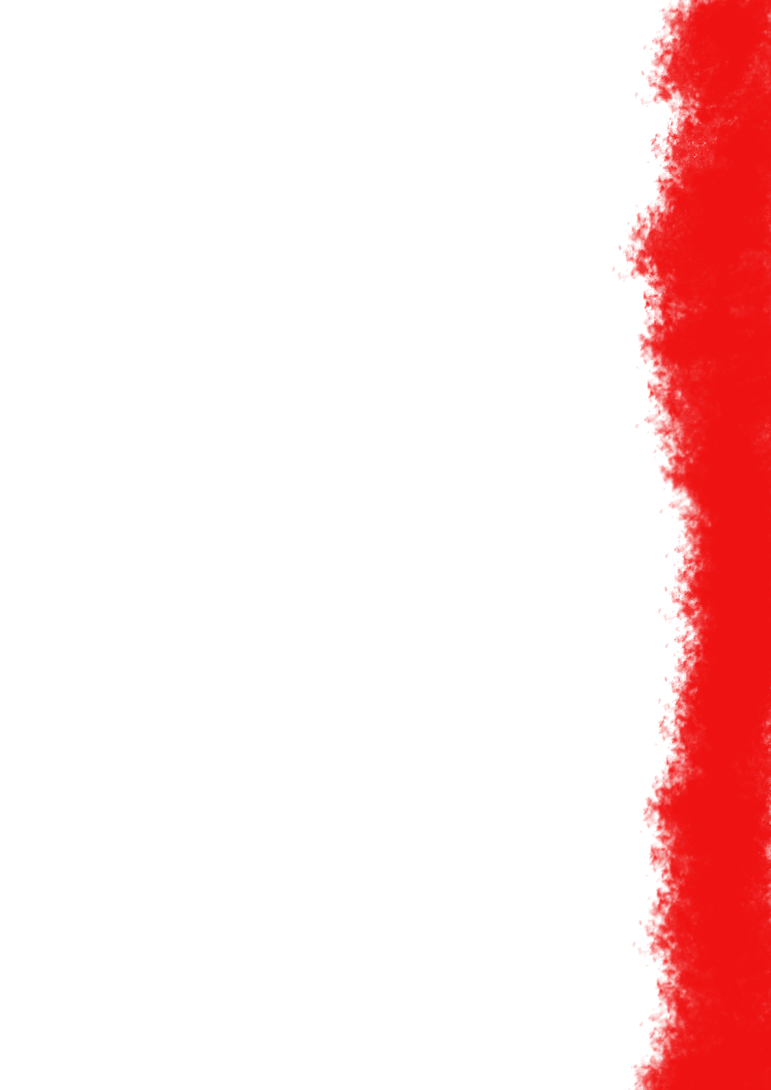
\includegraphics[scale=3.3]{watermarks/test-a.png}}	% página específica
%\newwatermark[oddpages]{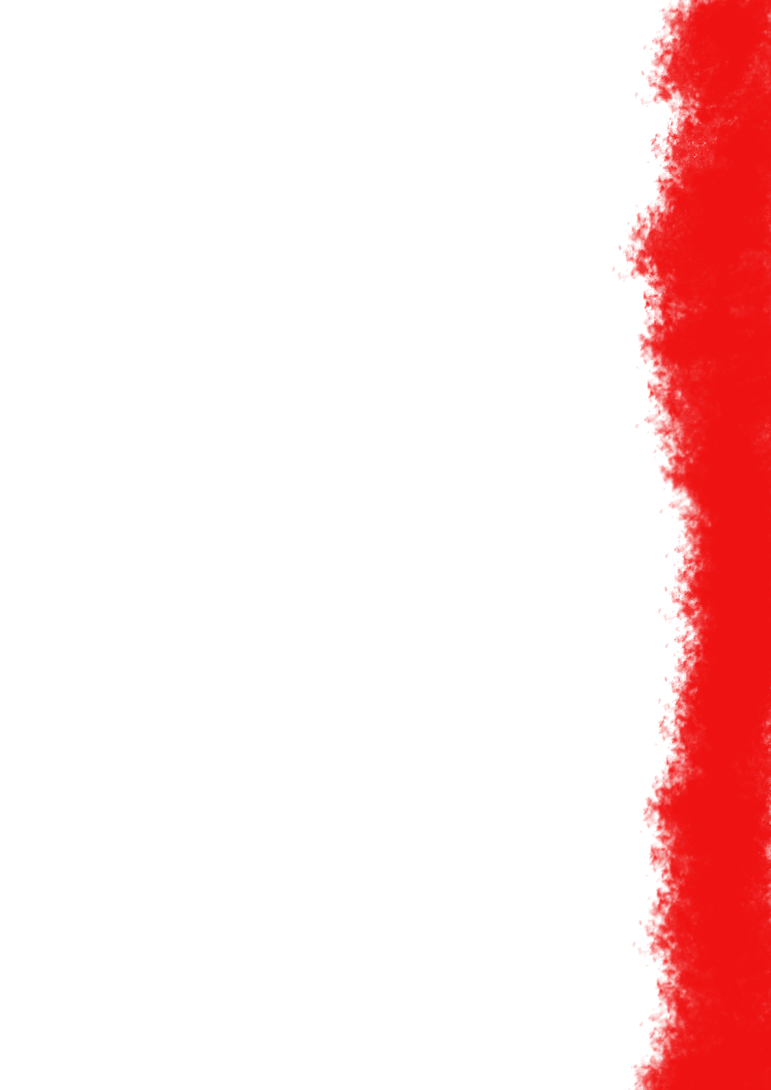
\includegraphics{watermarks/test-a.png}}			% páginas ímpars
%\newwatermark[evenpages]{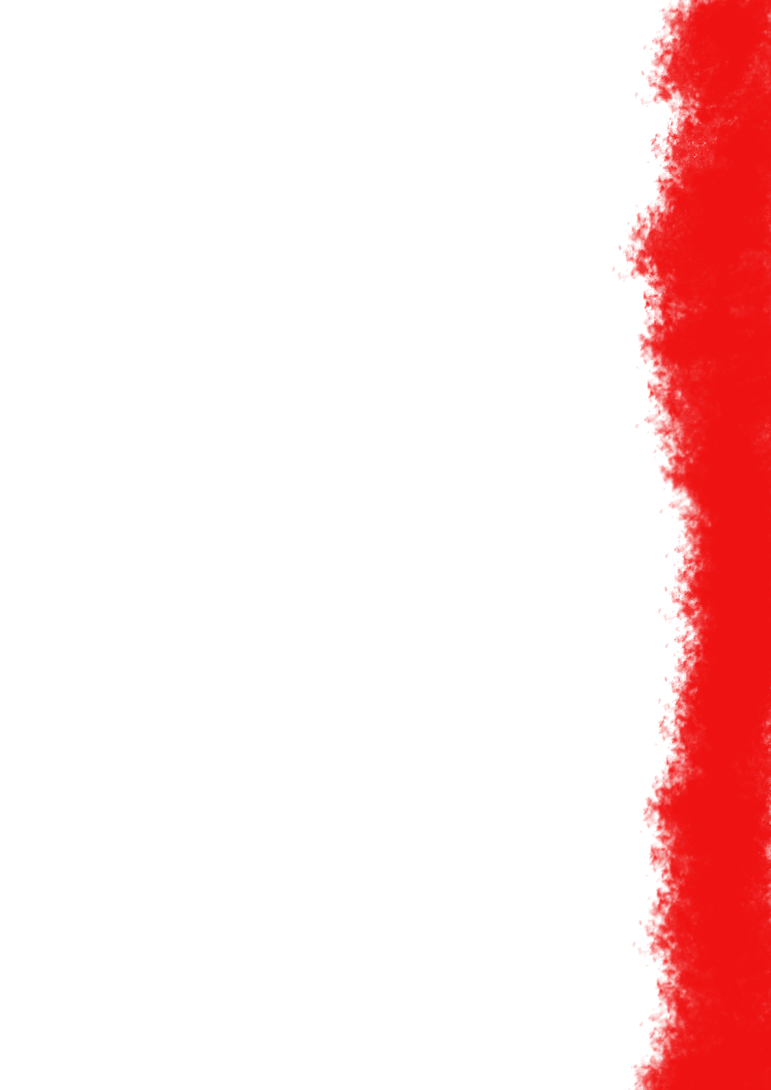
\includegraphics{watermarks/test-a.png}}			% págimas pares
\newwatermark[allpages]{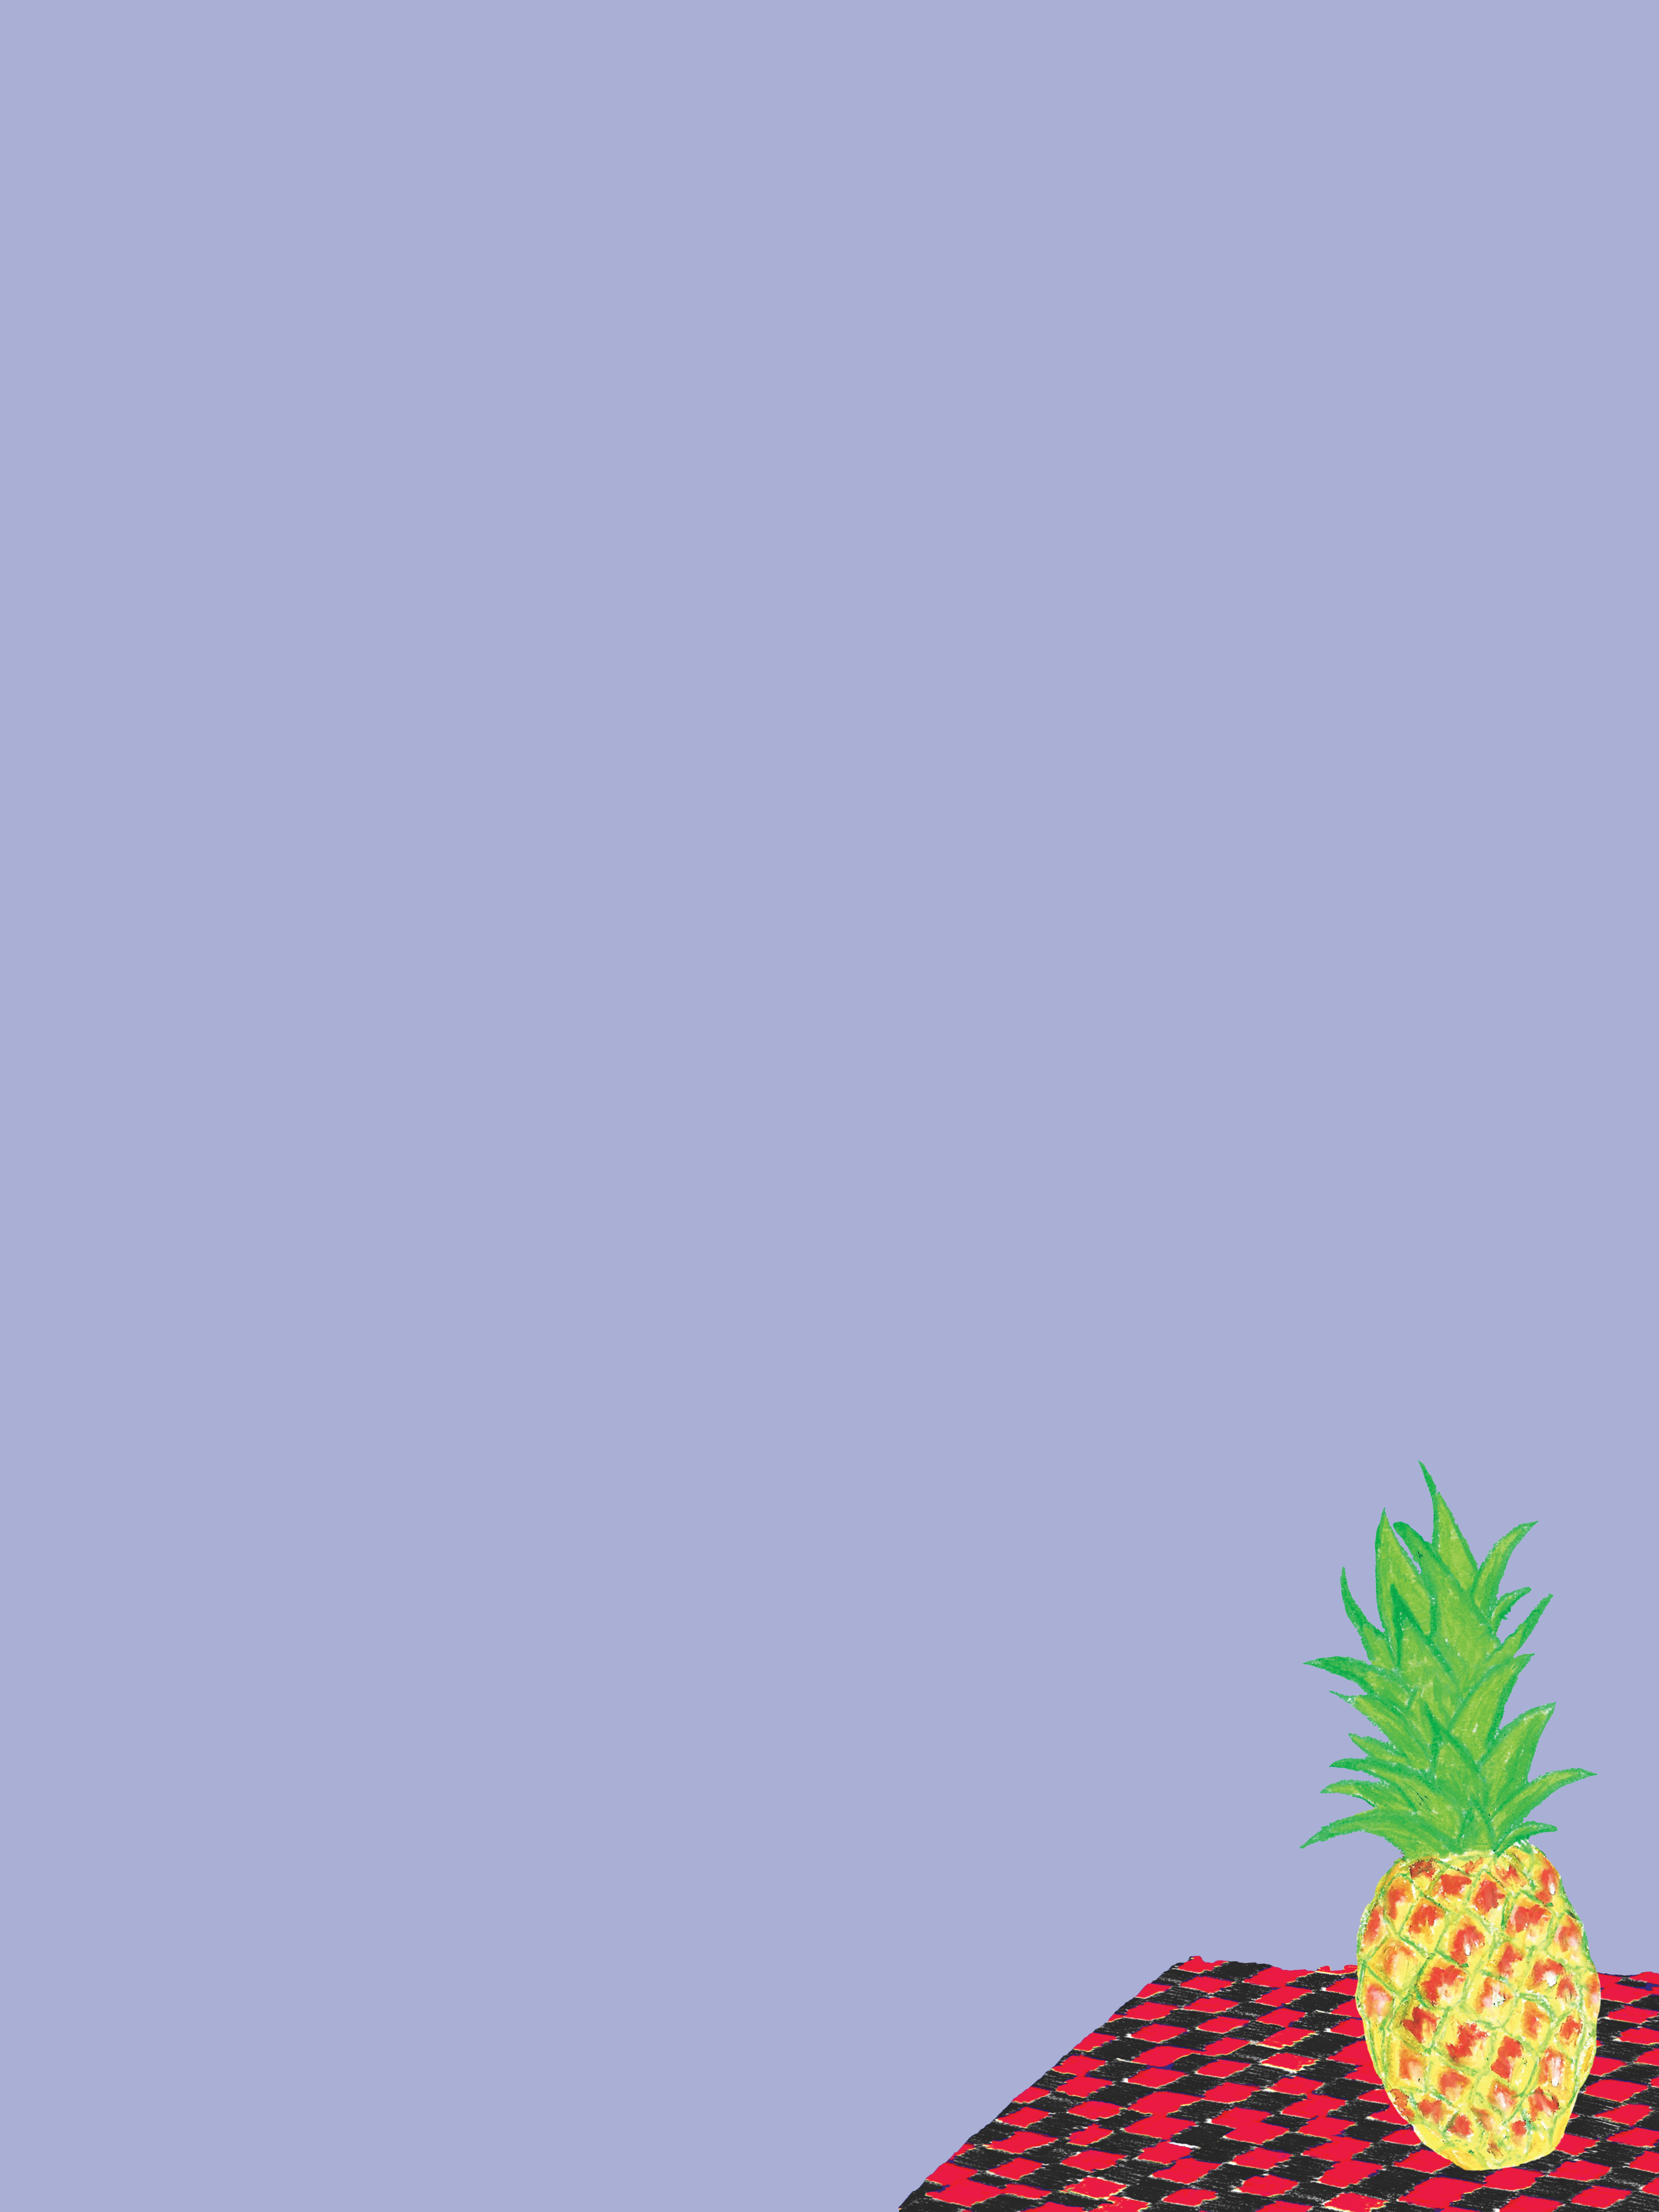
\includegraphics[scale=1]{watermarks/018.png}}

\pagecolor{cyan!0!magenta!10!yellow!28!black!28!}

\newcommand{\AutorLivro}{Camila Werner}
\newcommand{\TituloLivro}{Calu e as frutas}
\newcommand{\Tema}{Quotidiano de crianças nas escolas; nas famílias e nas comunidades (urbanas e rurais)}
\newcommand{\Genero}{Narrativos: fábulas originais; da literatura universal e da tradição popular; etc}
\newcommand{\imagemCapa}{./images/PNLD2022-018-01.pdf}
\newcommand{\issnppub}{978-65-99448-44-7}
\newcommand{\issnepub}{978-65-99448-46-1}
% \newcommand{\fichacatalografica}{PNLD0001-00.png}
\newcommand{\colaborador}{{Paulo Pompermaier e Renier Silva}}

\begin{document}

\title{\TituloLivro}
\author{\AutorLivro}
\def\authornotes{\colaborador}

\date{}
\maketitle

%\begin{abstract}\addcontentsline{toc}{section}{Carta ao professor}
%\pagebreak

\tableofcontents



\section{Sobre o livro}

%27 caracteres
\paragraph{O livro} 
``Calu e as frutas'' é um livro com uma narrativa em texto e imagem. 
%822 caracteres
\paragraph{Descrição} 
Calu conhece as frutas nacionais por meio dos gostos e costumes alimentares
de sua família. Cada um tem sua preferida e um modo específico de consumi-la.
Também é apresentada a proveniência das frutas: elas vêm do pomar. 
%411 caracteres
\paragraph{Competências} 
Com esta história, as crianças devem ser induzidas a uma relação
positiva com os alimentos provindos da natureza. As crianças terão
a oportunidade de compreender os processos básicos de produção
dos alimentos na medida em que elas conhecem, através do livro, o trajeto 
da fruta do pomar até a mesa. Além disso, poderão conhecer a diversidade
alimentar à disposição em suas comunidades.

%862 caracteres
\paragraph{Aprofundamento} 
Este material tem a intenção de contribuir para que você consiga desenvolver um trabalho aprofundado 
com esta obra na sala de aula. Você encontrará informações sobre o autor, sobre 
o gênero e sobre os temas trabalhados ao longo do livro. Apresentaremos também 
algumas propostas de trabalho para a sala de aula que você poderá explorar livremente, 
da forma que considerar mais apropriada para os seus estudantes. Para a prática 
da Literacia Familiar, oferecemos um guia que pode ajudar nas orientações aos 
responsáveis pela criança, para incentivar o gosto pela leitura e contribuir para 
que os estudantes desenvolvam em casa habilidades que serão importantes no momento 
da alfabetização. Por fim, você encontrará sugestões de livros, artigos e sites 
selecionados para enriquecer a sua experiência de leitura e, 
consequentemente, a de seus estudantes.


\section{Sobre o autor}


\paragraph{A autora}
Atua há 18 anos no 
mercado editorial brasileiro e internacional, com experiência 
em diversos segmentos como didático, literatura, trade, 
referência, acadêmico e infantojuvenil, entre outros. 

%313 caracteres
\paragraph{Publicações}
Publicou pela editora Hedra os seguintes livros: \emph{Bolotas e quadrados},
\emph{Esconde-esconde}, \emph{Bom dia, Calu}, \emph{Na casa de Calu}, \emph{Calu e os animais} e
\emph{Calu e as frutas}, todos voltados para o público infantil.

\reversemarginpar
\marginparwidth=5cm

\marginnote{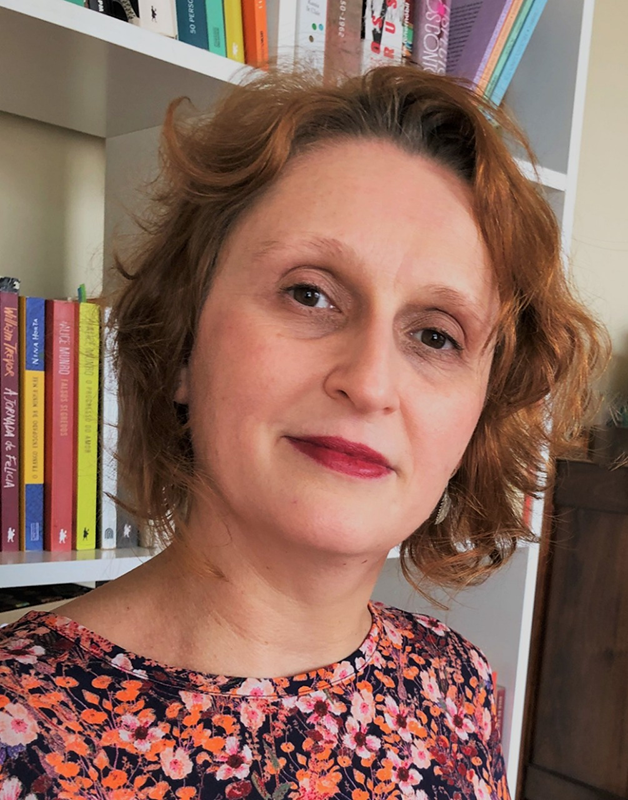
\includegraphics[width=\marginparwidth]{./images/PNLD2022-018-02.png}\\
A autora Camila Werner (Arquivo pessoal)\\\bigskip
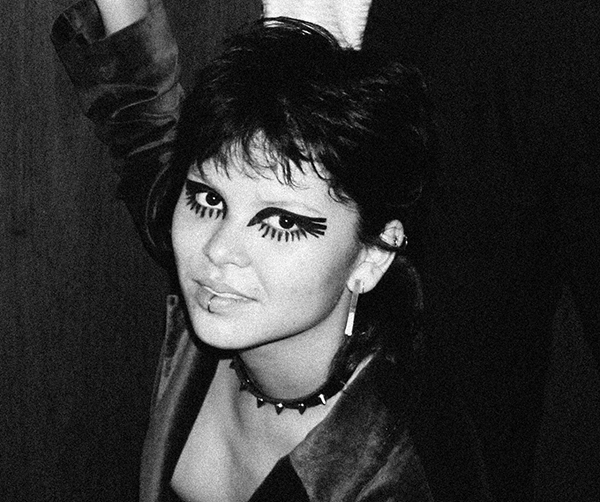
\includegraphics[width=\marginparwidth]{./images/PNLD2022-018-03.png}\\
A ilustradora Isabel Lee (Arquivo pessoal)}

%358 caracteres
\paragraph{Currículo} 
Formada em Comunicação Social com 
especialização em Produção Editorial pela \textsc{eca/usp} 
e mestrado em Books and Digital Media Studies pela 
Universidade de Leiden, Países Baixos.
Atualmente coordena o departamento digital da Brinque 
Book, editora especializada em livros infantojuvenis.
 


\section{Sobre o gênero}

%55 caracteres
\paragraph{O gênero} O gênero deste livro é \textit{narrativa}. 

%596 caracteres
\paragraph{Descrição} 
O gênero narrativo possui uma variedade de tipos e, cada um, suas estruturas específicas.
A característica comum entre todos é que sempre há uma história a ser contada, com linearidade,
ou seja, começo, meio e fim, e personagens. 
Dentre os tipos de narrativas mais comuns na literatura infantil, estão: mito, lenda, 
fábula e apólogo. Este último, semelhante à fábula, possui personagens não humanos, 
dramatização de fala, e uma moral, implícita ou explícita, mas difere na natureza destas 
personagens: se no caso da fábula se trata de animais, no caso do apólogo as personagens 
são objetos inanimados. No caso deste livro, a pinta de uma joaninha, que é mais um 
símbolo do que um objeto. Quase qualquer coisa pode ser uma personagem de uma narrativa 
infantil, já que a capacidade reflexiva das crianças nesta idade ainda está em um nível primário. 


%603 caracteres
\paragraph{Interação} 
As narrativas são uma forma de inserir os sujeitos no mundo. 
São elas que apresentam boa parte dos valores culturais da sociedade 
onde se vive. Mas não é só passivo o papel das crianças nesta experiência. 
As interações entre dois ou mais personagens onde se verifica
uma ação de linguagem organiza e impulsiona experiências compartilhadas,
importantes para o desenvolvimento psíquico do sujeito nos primeiros anos de vida.
Neste sentido, as narrativas são uma ótima ferramenta para
apresentar o mundo e capacitar as crianças para viver nele, mas como se
trata de um trabalho com a linguagem, sempre dando espaço à individualidade, 
seja na compreensão das histórias, na identificação com as personagens, ou 
no ato de narrar. 

\Image{O gênero da narrativa proporciona ao leitor uma abertura ao mundo. (Pixabay/Tumisu; CC-BY-2.0)}{PNLD2022-018-07.png}

%862 caracteres
\paragraph{Competências} 
Para além da narrativa, o livro apresenta às crianças uma linguagem artística complexa.
Explorar as cores, as formas, o posicionamento das personagens 
na página e até mesmo a opinião e os sentimentos das crianças sobre as imagens 
são possibilidades que aprofundarão a leitura, aumentarão o repertório 
e incentivarão o desenvolvimento do vocabulário e da fluidez do discurso. 

\section{Temas}

\subsection{Quotidiano de crianças nas escolas; nas famílias e nas comunidades (urbanas e rurais)}

%136 caracteres
\paragraph{Abordagem} 
São apresentadas frutas comuns no quotidiano das famílias brasileiras.
%206 caracteres
\paragraph{Descrição} 
A personagem principal conhece as frutas nacionais
por meio dos gostos e criações de sua família. 
%275 caracteres
\paragraph{Competências} 
Este tema relaciona-se, principalmente, mas não só, 
ao campo da experiência ``Espaços, tempos, quantidades e transformações''
descrito pela \textsc{bncc}, que explora a observação, o relato e a descrição 
de incidentes do cotidiano e fenômenos naturais.

\section{Modelagem de aula}
A seguir você encontrará a descrição de uma aula modelo como exemplo 
prático de exploração do livro com estudantes. Esta seção apresentará 
orientações sobre como organizar a sala de aula para receber os 
estudantes, exercitar a interação verbal e prepará-los para o 
momento da leitura.

Em seguida, você encontrará a \textbf{Leitura dialogada}, um 
tópico destinado a te orientar para o momento específico da 
leitura com os estudantes. Por fim, no tópico 
\textbf{Propostas de atividades}, você encontrará ideias 
de práticas que pode explorar com as crianças em sala de 
aula após a leitura. 

Essas atividades podem ser trabalhadas de acordo com a 
disponibilidade do seu cronograma e fique à vontade para adaptá-las 
da forma que achar melhor para os seus estudantes. Cada turma é única 
e o seu conhecimento prático das características de cada aluno será 
essencial para definir a melhor forma de aplicar essas ideias. 

O objetivo deste manual é oferecer algumas ideias 
e inspirações para um trabalho que pode ser desenvolvido tanto 
a curto, quanto a médio e longo prazo. Sinta-se a vontade para 
personalizar a aula e torna-la sua, aplicando seus conhecimentos, sua 
personalidade e aproveite para fortalecer 
seu vínculo com a turma.


\subsection{Antes de ler}

\BNCC{EI02ET02} 
\BNCC{EI02ET03} 
\BNCC{EI02ET04} 
\BNCC{EI02ET05}
\BNCC{EI02ET06} 


%Alterar o nível escolar nesse parágrafo.
Como este trabalho será realizado com crianças da \textbf{Creche \textsc{ii}}, 
que ainda não têm muita intimidade com o livro enquanto objeto, você terá o 
papel de mediar este contato. 

Nosso objetivo é que os próprios estudantes possam manusear 
e explorar o livro de forma autônoma, mas, para que isto aconteça, você 
pode ajudar a tornar o caminho mais convidativo com atividades que tenham 
intencionalidade educativa. 

A \textsc{bncc} define intencionalidade educativa como ``organização 
e proposição, pelo educador, de experiências que permitam às crianças 
conhecer a si e ao outro e de conhecer e compreender as relações com a 
natureza, com a cultura e com a produção científica, que se traduzem nas 
práticas de cuidados pessoais (alimentar-se, vestir-se, higienizar-se), 
nas brincadeiras, nas experimentações com materiais 
variados, na aproximação com a literatura e no encontro com as 
pessoas''.\footnote{\textsc{bncc}, página 39}

É importante manter essa intencionalidade em mente não apenas na condução 
das atividades propostas neste manual, mas também para aproveitar as 
oportunidades espontâneas de construir conhecimentos que podem surgir durante 
a interação direta com os estudantes.

\begin{enumerate}
%836 caracteres
\item \textbf{O ambiente}\quad Antes de iniciar o trabalho com o livro, é importante que você 
prepare o ambiente para receber a turma. Como o trabalho com o livro terá 
três momentos (antes, durante e depois da leitura), seria interessante que você 
criasse um ambiente para cada etapa. Nas \textbf{Sugestões de referências complementares} 
você encontrará um artigo que discorre sobre a importância da organização da sala 
de aula para a educação infantil, que pode ser um bom guia para a criação desses 
ambientes. Para o momento antes da leitura, você pode decorar a sala de aula
com diversas frutas em quantidade considerável. Organize-as em cestos
espalhados pelo ambiente. 

\Image{Para apresentar o livro, espalhe cestos de frutas pela sala de aula. (Pixabay; CC-BY-2.0)}{PNLD2022-018-09.png}

%413 caracteres
\item \textbf{Primeira opção}\quad Utilize os primeiros 
momentos da aula para passear pelo ambiente com as crianças.
Depois de ambientadas, pegue cada cesto de fruta e pergunte
quantas têm em cada um. Por exemplo, mostre-as quatro maçãs 
e pergunte: ``quantas tem aqui?''. Repita isso com todos
os tipos de fruta que houver. Conforme eles forem respondendo,
e caso demonstrem vontade, você pode oferecer para que comam. 

%632 caracteres
\item \textbf{Segunda opção}\quad Outra possibilidade para familiarizar 
as crianças com as frutas que serão abordadas no livro é trabalhar
com uma música infantil. Cada número deve ser representado por uma 
fruta que será exibida na hora da música. Por exemplo, no número um,
todos mostram uma banana, duas, no número dois, três, no número três,
e assim por diante. O educador pode fazer algumas brincadeiras como
trocar a ordem dos números para estimular as crianças. Ao fim, bem
como na primeira atividade, deixe que as crianças comam caso tenham vontade. 
\end{enumerate}


\subsubsection{A interação verbal} 
Criar situações em que as crianças precisam dialogar diretamente com 
você é uma das práticas mais importantes de Literacia, pois elas estimulam 
o desenvolvimento linguístico, ampliam o vocabulário e reforçam a 
capacidade dos estudantes de compreenderem o que ouvem e se expressarem 
pela fala. O diálogo livre com a criança também reforça sua autoestima, pois 
a faz se sentir ouvida e valorizada pelo adulto, ao vê-lo prestar atenção 
no que ela tem a dizer. Portanto, sempre que possível, reserve um tempo na 
aula apenas para a interação verbal. 

Como esse tipo de interação é espontânea e intimamente atrelada ao 
desenvolvimento de cada estudante, nossas orientações não serão específicas. 
A ideia é que você adapte este momento de acordo com as respostas e os 
repertórios das crianças. É um momento de estreitamento de vínculos e, portanto, 
fique a vontade para ser espontânea e para explorar os tópicos que achar 
mais interessantes para a sua turma.

Inicie as conversas com naturalidade, seguindo os objetos de atenção dos bebês. 
Você pode partir de objetos que estejam olhando ou sons que estão balbuciando 
para iniciar um assunto e incentivar que tentem se expressar. Ainda que nem 
todos os sons coincidam com palavras que conhecemos, continue interagindo, 
pois a intenção aqui é que o bebê perceba que outras pessoas estão respondendo 
à sua tentativa de comunicação. 

Fique atento a todas as formas de expressão: os gestos, as falas, as 
expressões faciais, para onde olham\ldots{} tudo pode ser explorado durante a conversa. 
Demonstre curiosidade sobre eles, seja um ouvinte entusiasmado e incentive que eles 
conversem entre si. Faça perguntas e construa a resposta junto com as crianças, 
a partir dos sons que eles emitem ou de informações que você saiba. 

A seguir, algumas dicas que podem contribuir para que a interação verbal 
seja produtiva em sua sala de aula: 

\begin{enumerate}
\item Sente-se no chão e brinque com eles, estabelecendo 
contato visual. Embora não consigam falar, vocalizações, 
gestos e expressões faciais podem ser boas formas de comunicar.

\item Não se esqueça que a conversa é uma troca e, portanto, 
evite ficar falando sozinho ou desvalorizar as respostas dos 
bebês porque não são palavras completamente articuladas. 
Nunca descarte uma tentativa de comunicação. 

\item Evite utilizar falas negativas que desencorajam o diálogo, 
como ``não pode!'', ``tire a mão'', ``não faça''. Se precisar que a turma 
corrija algum comportamento, explique claramente a razão e 
oriente com calma. Incentive positivamente as crianças e 
destaque o motivo de seus elogios. 

\item Aproveite alguns momentos durante a conversa para chamar 
a atenção das crianças para os sons das palavras e das letras que você 
acabou de usar ou que eles pronunciaram.  

\item Fale sempre com os bebês, pois, apesar de não conseguirem 
falar muito, são capazes de compreender muito.

\item Você pode utilizar a fala materna\footnote{Fala meiga, frequentemente 
utilizada com bebês e crianças pequenas, que alonga as 
vogais das palavras.}, mas não distorça 
a pronúncia correta das palavras e evite diminutivos. Interprete 
os gestos do bebê nomeando seus desejos verbalmente. Se você escutar 
alguma sílaba ou palavra, repita de volta completando e estimule 
positivamente as tentativas de fala. 

\item Explore possibilidades de interação como apontar e 
nomear objetos, pessoas e animais, imitar o bebê ou pedir que 
ele o imite, fazer caretas, jogar beijos, reproduzir sons de 
animais para que repitam, ensinar os nomes de partes do corpo, 
entre outras atitudes que estimulem a comunicação com a criança. 

\item Muitas dessas dicas poderão ser aproveitadas pela 
família durante a prática da Literacia Familiar. Portanto, 
se achar necessário, compartilhe algumas destas orientações 
com as famílias dos estudantes.
\end{enumerate}


\subsection{A leitura dialogada}
Este é o momento em que será realizada a leitura propriamente dita. 
Se possível, crie um \textit{cantinho da leitura} em sua sala de aula. Um 
ambiente confortável, de preferência em que todos se sentem no chão ou 
em pufes para que consigam enxergar as ilustrações do livro que está 
sendo lido e interagir com facilidade. Se houver possibilidade, mantenha 
sempre os livros da turma em uma altura da estante que permita fácil 
acesso para os estudantes ou guarde os livros em uma caixa que as crianças 
possam mexer com autonomia. É importante que elas tenham autonomia para 
acessar os livros e se sintam à vontade para pegá-los sempre que quiserem. 

\Image{É importante que o cantinho da leitura proporcione autonomia para as crianças. (Fotos Públicas/Marina Cajaíba; CC BY-NC 2.0)}{PNLD2022-018-08.png}

Outra possibilidade de ambiente para esta leitura, se a escola permitir, 
é efetuar essa leitura ao ar livre, embaixo de uma árvore, onde as crianças 
possam ouvir os sons dos pássaros e sentir o cheiro da grama. Sair da sala 
de aula pode oferecer um ótimo leque de experiências aos seus estudantes e 
reforçar a conexão entre a natureza do livro e a realidade.  

Reserve uma boa parte da aula para o momento da leitura com os estudantes, 
pois é importante que esse momento aconteça sem pressa. O objetivo da 
leitura dialogada é que seja uma leitura em bate-papo. A criança deve 
assumir um papel ativo na leitura, mesmo que ainda não seja capaz de 
ler sozinha. Além de promover o gosto pela leitura, esta prática estimula 
o desenvolvimento da linguagem, enriquece o vocabulário e 
aumenta o conhecimento de mundo.

%Especificar o livro.
No caso de “Calu e as frutas” o diálogo durante a leitura é 
importante para que as crianças tomem consciência de que aqueles
nomes e ilustrações são elementos que fazem parte de suas vidas
em casa e na escola. O educador deve estimular esta compreensão por meio
do diálogo.
Você deve interagir com eles durante toda a 
leitura, fazendo perguntas e partindo de detalhes do livro para 
levantar novas questões. 

A seguir, algumas orientações para aproveitar este momento: 

\begin{enumerate}
%177 caracteres
\item \textbf{Como começar}\quad Sente-se em um lugar acessível, 
onde todos conseguirão ouvir bem a sua leitura e enxergar as ilustrações 
quando você estiver mostrando o livro ou eles estiverem manuseando-o. 
Antes de abrir o livro, chame a atenção dos estudantes para a capa. 
Faça perguntas sobre a capa, como: 

\begin{itemize}
\item O que é isso na capa?
\item É de comer?
\item Quem já comeu?
\item Quais outras frutas existem?
\end{itemize}

Estas perguntas ajudarão a introduzir ao assunto que será tratado. 
É importante começar a sugerir que vocês vão falar de comida,
e que existem vários tipos de frutas com gostos
e nomes diferentes. Se achar 
conveniente, peça que repitam algumas palavras com você e valorize tentativas 
de imitar a sua fala. 
 
%230 caracteres
\item \textbf{Manuseio}\quad Deixe que as crianças manuseiem o livro 
e explore com elas todos os elementos que o compõe. Mostre o que é a 
capa e onde estão as páginas. Leia o título do livro em voz alta, seguindo 
a leitura com o dedo, indicando as letras. 

%495 caracteres
\item \textbf{Diálogo}\quad A cada página ou a cada nova fruta,
chame a atenção dos alunos para ele. Faça perguntas como:

\begin{itemize}
\item Que fruta é essa?
\item Quem gosta?
\item Quem já comeu?
\item É doce ou azedo?
\end{itemize}

Se os estudantes não conseguirem responder, explique ou mostre uma 
imagem ou um vídeo. Traga referências além da ilustração e da frase. 
Incentive-os a relatar experiências com esses objetos.

%346 caracteres
\item \textbf{Escuta}\quad Elogie atitudes positivas, como 
tentar tomar o papel central na leitura. Se os estudantes tentarem 
tomar o seu lugar e começar a narrar a história --- com palavras já articuladas 
ou não --- valorize e escute com atenção o que estiverem falando. Mas não 
force a leitura. Se as crianças estiverem cansadas, faça outra atividade 
e retorne depois. 

\includepdf[nup=2x3, 				% grid
			%offset=-15mm -5mm, 	% posição
			scale=.8, 				% tamanho da página
            delta=4mm 4mm, 			
            frame,
            pages={12-13,14-15,22-23}]{./pdfs/\jobname_MIOLO.pdf}


%935 caracteres
\item \textbf{Leitura}\quad Faça perguntas e comentários que aumentem o 
interesse e aticem a curiosidade das crianças sobre a história. Faça 
perguntas ou comentários como: 

\begin{itemize}
\item Qual será a fruta que a mãe de Calu gosta?
\item E a que ela não gosta?
\end{itemize}

Não tenha pressa em passar as páginas.
A intenção é que seja uma leitura com bastante comentários
da parte das crianças, que devem contribuir com nomes de 
frutas já conhecidas em seu ambiente familiar.

Não deixe que eles fiquem sem entender do que se trata alguma que
por ventura não conheçam. Crie 
um ambiente amigável onde a criança se sinta à vontade para fazer 
perguntas e comentários durante a leitura.


%382 caracteres
\item \textbf{Interação}\quad Nomeie os elementos das ilustrações 
do livro, apontando para elas com o dedo. Destaque os sons de algumas 
palavras. Interrompa a leitura em alguns momentos e peça que 
os estudantes repitam palavras, como \textit{abacaxi}, \textit{pitanga}, \textit{morango}. Se possível, 
leia a mesma história várias vezes ou explore as imagens em uma ordem 
diferente, construindo uma nova narrativa com os estudantes. 
\end{enumerate}


\subsection{Propostas de atividades}

\BNCC{EI02ET02} 
\BNCC{EI02ET03} 
\BNCC{EI02ET04} 
\BNCC{EI02ET05}
\BNCC{EI02ET06} 
\BNCC{EI02EF09}

\begin{enumerate}
%700 caracteres
\item \textbf{Contexto}\quad Após a leitura dialogada, é hora de criar 
atividades que proporcionem aos estudantes experiências novas a partir da história 
que acabaram de conhecer. Nesta idade é fundamental explorar os sentidos da criança e 
ajudá-lo a experimentar a história que acabou de conhecer de formas diversas. Se achar 
conveniente, convide os estudantes a se sentarem nas carteiras para este terceiro 
momento, pois muitas atividades que serão realizadas exigem apoio para escrever 
ou manipular objetos. É interessante, por exemplo, que a criança perceba a conexão 
entre as imagens que acabou de ver e os elementos da realidade. Para ajudar a traçar 
essa relação, separe previamente objetos da natureza relacionados ao livro. 

\item \textbf{Materiais}\quad Recipientes reutilizados (garrafa \textsc{pet}, 
embalagem de leite, uma banda de côco\dots{}), algodão, um pouco de terra, sementes
de frutas para plantar, papel e fita adesiva.

%650 caracteres
\item \textbf{Ambiente}\quad Pomar da escola, caso haja, ou alguma horta
nas proximidades. Fazer uma visita com as crianças ao espaço. Se não for 
possível, um ambiente externo com alguma árvore pode ser utilizado. 

%950 caracteres
\item \textbf{A atividade}\quad Em ``Calu e as frutas'' as crianças 
conheceram algumas das frutas mais populares no Brasil e descobriram 
que elas vêm do pomar. Para trabalhar as noções de temporalidade,
transformação, causa e consequência com os pequenos, sugerimos que
o educador apresente às crianças sementes de frutas, 
de preferência aquelas às quais foram apresentadas no livro: 
melancia, laranja, maçã, limão, morango, pintanga\dots{}
Se possível, mostre-lhes onde elas estão nas frutas. Explique
que toda fruta tem uma semente dentro dela. 
Então, cada um deve encher seu recipiente de terra, colocar
a semente de sua preferência e aguar. 
O educador deve mostrar às crianças as árvores
que dão frutos, seja pessoalmente no pomar ou por meio de 
imagens, e então explicá-las que, um dia, a semente que plantaram
pode transformar-se numa árvore como aquela e também ela dar outros 
frutos. 
Para finalizar, cada criança deve escrever seu nome num papel
e colar no recipiente, que deve ficar num espaço que receba luz solar. 
Adverta-os que as plantas começarão a nascer nas próximas semanas. 

\Image{É interessante que as crianças associem as frutas às árvores de onde vêm. (Pxhere; Domínio público)}{PNLD2022-018-10.png}

%550 caracteres
\item \textbf{Interação}\quad O livro pode e deve ser 
manipulado pelos estudantes. Incentive que eles contem a história para 
você, faça perguntas como \emph{Do que o pai de Calu gosta? E o avô?
Quais as frutas que Calu gosta de comer?}
Caso confundam algum nome com a ilustração, não hesite em corrigi-los. 
Peça que repitam algumas palavras para ajudar a fixá-las.
\end{enumerate}


\section{Literacia familiar}
O \textsc{pna} dá destaque especial para a importância do envolvimento da família 
no processo pedagógico nesta faixa etária e denomina Literacia Familiar o conjunto 
de experiências e práticas relacionadas à linguagem (oral, escrita ou lida) vivenciadas 
com os cuidadores. 

Essas estratégias podem começar a ser colocadas em prática desde a 
gestação e continuar até o final da adolescência. São práticas simples e divertidas 
que estimulam o desenvolvimento de quatro atividades fundamentais: ouvir, falar, 
ler e escrever que criam momentos de afeto e interação para a família. 

Para que esse trabalho conjunto entre escola e família funcione, é 
fundamental que a escola esteja em constante diálogo com os responsáveis e 
você consiga orientá-los. Um grupo em aplicativos de mensagens instantâneas ou um 
grupo de e-mails são saídas viáveis para que a comunicação se estabeleça e pode ser 
uma forma útil das famílias compartilharem suas vivências e trocarem sugestões 
de abordagens, sempre contando com a sua mediação. 

Com o objetivo de incentivar 
a prática da \textit{literacia familiar}, se possível, organize um rodízio entre os familiares 
das crianças para emprestar o livro da biblioteca da turma. Neste caso, crie um caderno 
de registro e estabeleça períodos para cada família ficar com o livro. É importante 
que os familiares compreendam a seriedade deste compromisso, pois o livro pertence 
ao acervo da sala e, portanto, deve ser bem cuidado e devolvido na data acordada. 

Se não for possível garantir o acesso direto dos cuidadores da criança ao livro, 
grave um vídeo direcionado a eles, contando a história e apresentando algumas 
das ilustrações. O importante é que os familiares saibam com clareza qual livro 
está sendo trabalhado, a história contada e se sinta seguro para explorar as temáticas 
do livro com a criança. Orientações claras e a manutenção do canal de comunicação com 
os responsáveis é essencial para que eles se sintam seguros e à vontade para fazer perguntas 
se tiverem dúvidas. 

Neste manual, você encontrará algumas práticas que podem ser 
recomendadas aos familiares para ajudá-los a expandir e aprofundar o trabalho 
que você iniciou em sala de aula.


\subsection{Importância da leitura}
Na escola, aprendemos a ler letras, mas é importante ter em mente que nós 
lemos o mundo desde muito pequenos: “lemos” os animais que passam pelos nossos 
quintais, a expressão no rosto dos nossos familiares, as cores que pintam o céu 
em um fim de tarde. 

Vamos aprendendo, ao longo da vida, a interpretar acontecimentos 
e sons que escutamos e a utilizá-los para nossa comunicação. Aprender a ler textos e 
escrevê-los expande a nossa leitura do mundo, pois permite que sejamos capazes de 
interpretar um código e experimentar, a partir dele, novas experiências e conhecimentos. 

O simples contato com os livros já permite um leque grande de sensações: 
sentimos as texturas, as formas, vemos as cores do livro, escutamos o som da página 
virando e o som da voz do narrador, se a história estiver sendo lida em voz alta. Para um 
bebê, são experiências que podem contribuir diretamente com o desenvolvimento psicomotor 
e cognitivo. 

Nosso papel, enquanto mediadores de leitura, é contribuir para que essas 
sensações sejam associadas a momentos positivos, de construção de 
conhecimento e exercício de imaginação. 

Com os livros, podemos conhecer mais da história humana, descobrir informações 
novas sobre sociedades diferentes da nossa, imaginar situações e contextos inéditos 
para nós e aumentar o nosso repertório. São por meio deles que melhoramos nossa 
capacidade de interpretação, de expressão, de análise e senso crítico. Boas habilidades 
leitoras podem contribuir para o desenvolvimento de um estudante em todas as outras 
disciplinas, pois exercem influência direta na forma como absorvemos e 
construímos conhecimento.


\subsection{O papel da família na formação do leitor}
A família é peça fundamental na formação do leitor, pois é ela quem primeiro 
ensina a criança a ler. Não apenas os textos escritos, mas a ler o mundo, a 
interpretar os estímulos que a cercam, a construir seu próprio vocabulário e a 
comunicar seus pensamentos e necessidades. Na fase em que estão, os bebês 
absorvem o conhecimento com voracidade e tentam aprender a se comunicar. 

O universo das letras é muito presente na vida das crianças antes mesmo de sua 
entrada na escola. Aparece nas histórias e ilustrações do livro que o cuidador 
lê ao colocá-la para dormir, nas situações em que vê os responsáveis se comunicarem 
pela escrita ou nos textos que podem permear seu cotidiano (nos outdoors, na 
televisão, no celular, manuais de instrução entre outros). 

Os familiares têm, 
portanto, uma ótima oportunidade de apresentar a leitura com leveza, de forma 
prazerosa, associado ao contexto em que a criança vive e à momentos de diversão. 
Você poderá orientar os pais nesta tarefa, ensinando-os com este guia a aproveitar 
as oportunidades para trabalhar a Literacia com a criança.


\subsubsection{Práticas de literacia familiar} 

São muitas as experiências que a prática da \textit{literacia familiar} 
pode oferecer às crianças. A seguir, explicamos cada uma delas para que você possa, 
se achar necessário, compartilhar com os responsáveis enquanto estiver orientando-os: 

\paragraph{Interação verbal} Aumentar a quantidade de conversas com as 
crianças, fazendo perguntas para incentivar o diálogo.

\paragraph{Leitura dialogada} Interagir com a criança durante a leitura 
em voz alta, criar expectativa sobre o livro, chamar a atenção para detalhes 
das ilustrações e comentar o enredo.

\paragraph{Narração de histórias} Interagir com a criança enquanto 
estiver narrando uma história, por exemplo, incluindo-a na ação, utilizando 
marionetes ou permitindo que ela complete a narrativa.

\paragraph{Contatos com a escrita} Apresentar as letras para as 
crianças, incentivar que tentem escrever ou ler, ajudá-los a desenhar letras, 
entre outras formas de incentivar o contato com as palavras.

\paragraph{Atividades diversas} Qualquer atividade com a criança 
pode ser utilizada para contribuir para a alfabetização. Jogos, brincadeiras, 
instrumentos musicais, canto, dança, passeios e viagens oferecem boas 
oportunidades de aprendizado.

\paragraph{Motivação} Atitudes que motivem as crianças à envolver-se com 
o mundo da leitura e da escrita.

\subsection{Exercitando a literacia familiar}

\BNCC{EI02ET03} 
\BNCC{EI02EF07} 
\BNCC{EI02EF08} 
\BNCC{EI02EF03} 
\BNCC{EI02EF05} 

\begin{enumerate}
%700 caracteres
\item \textbf{Como começar}\quad Como o livro não apresenta 
texto verbal, apenas visual, é possível que os familiares se sintam 
perdidos sobre como explorá-lo com o bebê. Esclareça que a narrativa 
em imagens tem muitas potencialidades e permitirá o exercício da imaginação 
de forma muito ampla ao longo da leitura com o bebê pois as ilustrações são 
abertas à interpretação. Esse fato garantirá muito mais autonomia e 
envolvimento da criança na narrativa, pois ela poderá ter papel ativo na 
história que construirão juntos. Se achar conveniente, compartilhe com 
os familiares algumas dicas das seções Interação verbal 
e Leitura dialogada e as indicações nas Referências Complementares 
para ajudá-los a explorar as possibilidades oferecidas pelo livro. 

%650 caracteres
\item \textbf{Leitura}\quad A família pode continuar 
explorando os temas apresentados pelo livro. Os familiares podem explorar 
elementos do cotidiano que se relacionam à história e indicar a conexão 
com a realidade. A história de “Calu e as frutas” fala dos hábitos
alimentares de uma família e os familiares podem aproveitar este fato 
para compartilhar com a criança estes fatos. Os adultos cuidadores
podem pedir às crianças que escrevam os nomes dos familiares e suas frutas
favoritas, como: 
\begin{itemize}
	\item Tio João - abacaxi
	\item Vovô - caju
	\item Vovó - morango
\end{itemize}
Além disso, podem ressaltar as transformações que as frutas sofrem 
na alimentação da criança em seu quotidiano. Por exemplo, 
a laranja vira o suco de laranja, mas também pode ser chupada 
\emph{in natura}, a banana pode virar vitamina, e assim por diante. 

%1073 caracteres
\item \textbf{Instrução}\quad Informe aos pais que a 
história do livro de Taisa Borges é inspirada pela fábula “A águia e a coruja” 
de Leonardo da Vinci e oriente-os a ler esta fábula em voz alta para os 
bebês. Ela pode ser encontrada facilmente na internet. Desta forma as 
crianças terão contato com a mesma história em dois suportes narrativos 
diferentes. Mesmo pequenas, as crianças conseguem perceber a diferença entre 
as formas de contar, e elementos de uma linguagem podem ajudá-la a compreender 
sentidos e perceber detalhes de outra. Se possível, depois da leitura, oriente 
que voltem às imagens e recontem a história com o apoio das 
ilustrações. 

Outra opção é entregar o livro para a criança e pedir que ela conte 
a história para que o familiar ouça. Mesmo que a narrativa não pareça 
completa para o adulto, é importante que ele ouça com atenção e 
valorize todas as tentativas da criança. Afinal, ao tentar recontar, 
ela manipulará o livro, treinará a coordenação motora, conhecerá as texturas 
do objeto e poderá imitar a forma como o adulto 
conta a história, treinando a fala. 
\end{enumerate}

 
\section{Sugestões de referências complementares}

\subsection{Livros} 

\begin{itemize}
\item LINS, Guto. Livro infantil? projeto gráfico, metodologia, subjetividade. São Paulo: Rosari, 2002.
Livro que aborda a importância das escolhas visuais (ilustração, projeto gráfico, lettering) na literatura infantil.  

\item HUNT, Peter. Crítica, teoria e literatura infantil. São Paulo: Cosac Naify, 2010.
Livro sobre crítica de literatura infantil que contêm definições de livro ilustrado e livro imagem. 
\end{itemize}

\subsection{Artigos}

\begin{itemize}

	\item \textsc{carvalho}, Lydiane Fonseca de. \emph{Poesia na sala de aula: as contribuições da poesia na formação
	do leitor literário.} Disponível em: \url{http://www.cchla.ufrn.br/shXIX/anais/GT12/POESIA_ARTIGO_HUMANIDADES.pdf}. Acesso em 23 ago. 2021.
	Artigo acadêmico que discorre sobre as contribuições da poesia na formação de crianças.
	\item \textsc{sardelich}, Maria Emilia. \emph{Leitura de Imagens, Cultura Visual e Prática Educativa.} 
In: Cadernos de Pesquisa. V.36, n.128, p.451-472, mai/ago.2006. Disponível em: \url{https://www.scielo.br/pdf/cp/v36n128/v36n128a09}. 
Acesso em 29 abr 2021. 
Artigo acadêmico que discorre sobre a importância de trabalhar cultura 
visual na educação na sociedade contemporânea. 

\item \textsc{pranke}, Marha Elfrida. \emph{Organização dos espaços da sala de aula na Educação Infantil.} Disponível em: 
\url{http://centraldeinteligenciaacademica.blogspot.com/2016/04/organizacao-dos-espacos-da-sala-de-aula.html}. Acesso em 04 mai 2021. 
Artigo acadêmico que discorre sobre a importância da rotina e de criar ambientes dentro da sala de aula na Educação Infantil.  
\end{itemize}

\subsection{\textit{Sites}}

\begin{itemize}
\item Vídeos “Conta pra mim” no site do PNA. Disponível em: \url{http://alfabetizacao.mec.gov.br/contapramim}. 
Acesso em 13 abr. de 2021.
Página do MEC com vídeos sobre leitura dialogada que visam incentivar a Literacia Familiar. Muitas das 
técnicas, explicações e materiais disponíveis nessa página podem ser utilizados em aula, mas o site também 
pode ser uma ótima indicação para ajudar a direcionar os cuidadores dos estudantes a praticar 
a literacia familiar e leitura dialogada.

\item Vídeo “Livros de imagem: como utilizar com as crianças?” do canal Conta Outra. Disponível em Youtube. 
Acesso em 14 abr. 2021. 
Neste vídeo, a pedagoga Bel explica o que são livros de imagem e faz sugestões para mediar a leitura com 
crianças. Se você achar conveniente, esse vídeo pode ser recomendado aos familiares da criança 
para inspirá-los na leitura dialogada. 

\end{itemize}

\subsection{Para os estudantes}
\begin{itemize}
\item Música ``As Coisas'' do canal Arnaldo Antunes. Disponível em Youtube. Acesso em 23 ago. 2021. 
Nesta canção pop, o poeta chama atenção ao fato de que as coisas nunca são uma coisa só,
por isso nunca estão em paz. A melodia divertida deve ajudar as crianças a entrar no clima
criativo da canção. 

\item Música ``As Árvores'' do canal Arnaldo Antunes. Disponível em Youtube. Acesso em 23 ago. 2021.
Canção pop feita de um poema de Arnaldo Antunes, a letra adentra o universo das árvores, 
narrando poeticamente sua experiência no mundo. 

\item Livro de poesia ``As Coisas'' de Arnaldo Antunes. Escrito em 1991, este livro está em 
diálogo com as “Frases do Tomé aos três anos”. Aqui, Arnaldo Antunes trabalha com Rosa, sua 
filha então com a mesma idade de Tomé, três anos, só que na posição contrária. Se naquele 
caso o poeta fez as ilustrações para as frases do filhos, agora é a filha quem ilustra os 
poemas do pai. Bastante similar na abordagem – os poemas de As coisas buscam explicar as 
coisas existentes no mundo a partir de um olhar poético que encontra e constrói relações 
e sentidos fora do óbvio quotidiano – , este livro é um ótimo complemento para a leitura 
do primeiro. A infância e a poesia continuam de mãos dadas. 

\end{itemize}


\section{Bibliografia comentada}

\subsection{Livros}
\begin{itemize}
\item \textsc{brasil}. Ministério da Educação. Base Nacional Comum Curricular. Brasília, 2018.
Consultar a BNCC é essencial para criar atividades para a turma. Além de especificar 
quais habilidades precisam ser desenvolvidas em cada ano, é fonte de informações sobre 
o processo de aprendizagem infantil. 

\item \textsc{brasil}. Ministério da Educação. Secretaria de Alfabetização. Conta pra mim: Guia de Literacia Familiar. 
Brasília: MEC, SEALF, 2019. Disponível em: \url{http://alfabetizacao.mec.gov.br/images/conta-pra-mim/conta-pra-mim-literacia.pdf}
Este guia é voltado aos pais e oferece explicações em uma linguagem bastante acessível e detalhada as práticas de Literacia Familiar, 
como praticar leitura dialogada, como narrar histórias, como exercitar interação oral, formas de proporcionar contatos com a escrita à criança etc. 
 
\item \textsc{brasil}. Ministério da Educação. Secretaria de Alfabetização. PNA Política Nacional de Alfabetização/Secretaria 
de Alfabetização. Brasília: MEC, SEALF, 2019.
Um guia fundamental para trabalhar pré-alfabetização e alfabetização de estudantes, que ressalta a importância da Literacia e da Numeracia. 


\end{itemize}

\subsection{Artigos}

\begin{itemize}
\item \textsc{costa}, A. C. C.; \textsc{santos netos}, J. A.; \textsc{bortolin}, S; \textsc{pereira}, Ana Paula. O livro de imagem e a mediação na escola. 
In \textsc{vii secin}, Universidade de Londrina. Disponível em \url{http://www.uel.br/eventos/cinf/index.php/secin2017/secin2107/paper/viewFile/445/296}. 
Acesso em 29 abr 2021. 
Esse artigo reflete sobre a importância de se apresentar livros de imagem para os estudantes na escola para que as crianças aprendam a ler imagens. 

\item \textsc{nannini}, P. B. R.; \textsc{medeiros}, J. P. S.; \textsc{ribeiro}, J. M. Leitura em cena: Vivências em sala de aula com livro de imagens. 
Literartes, n. 3, p. 82-101, 2014. DOI: 10.11606/issn.2316-9826.literartes.2014.89204. 
Disponível em \url{https://www.revistas.usp.br/literartes/article/view/89204/92115}. Acesso em 29 abr. 2021. 
Artigo acadêmico sobre um trabalho utilizando o mesmo livro de imagem com crianças da educação infantil e ensino médio. 
É uma forma interessante de perceber que a leitura de imagens pode ser explorada com qualquer faixa etária. 
\end{itemize}

% 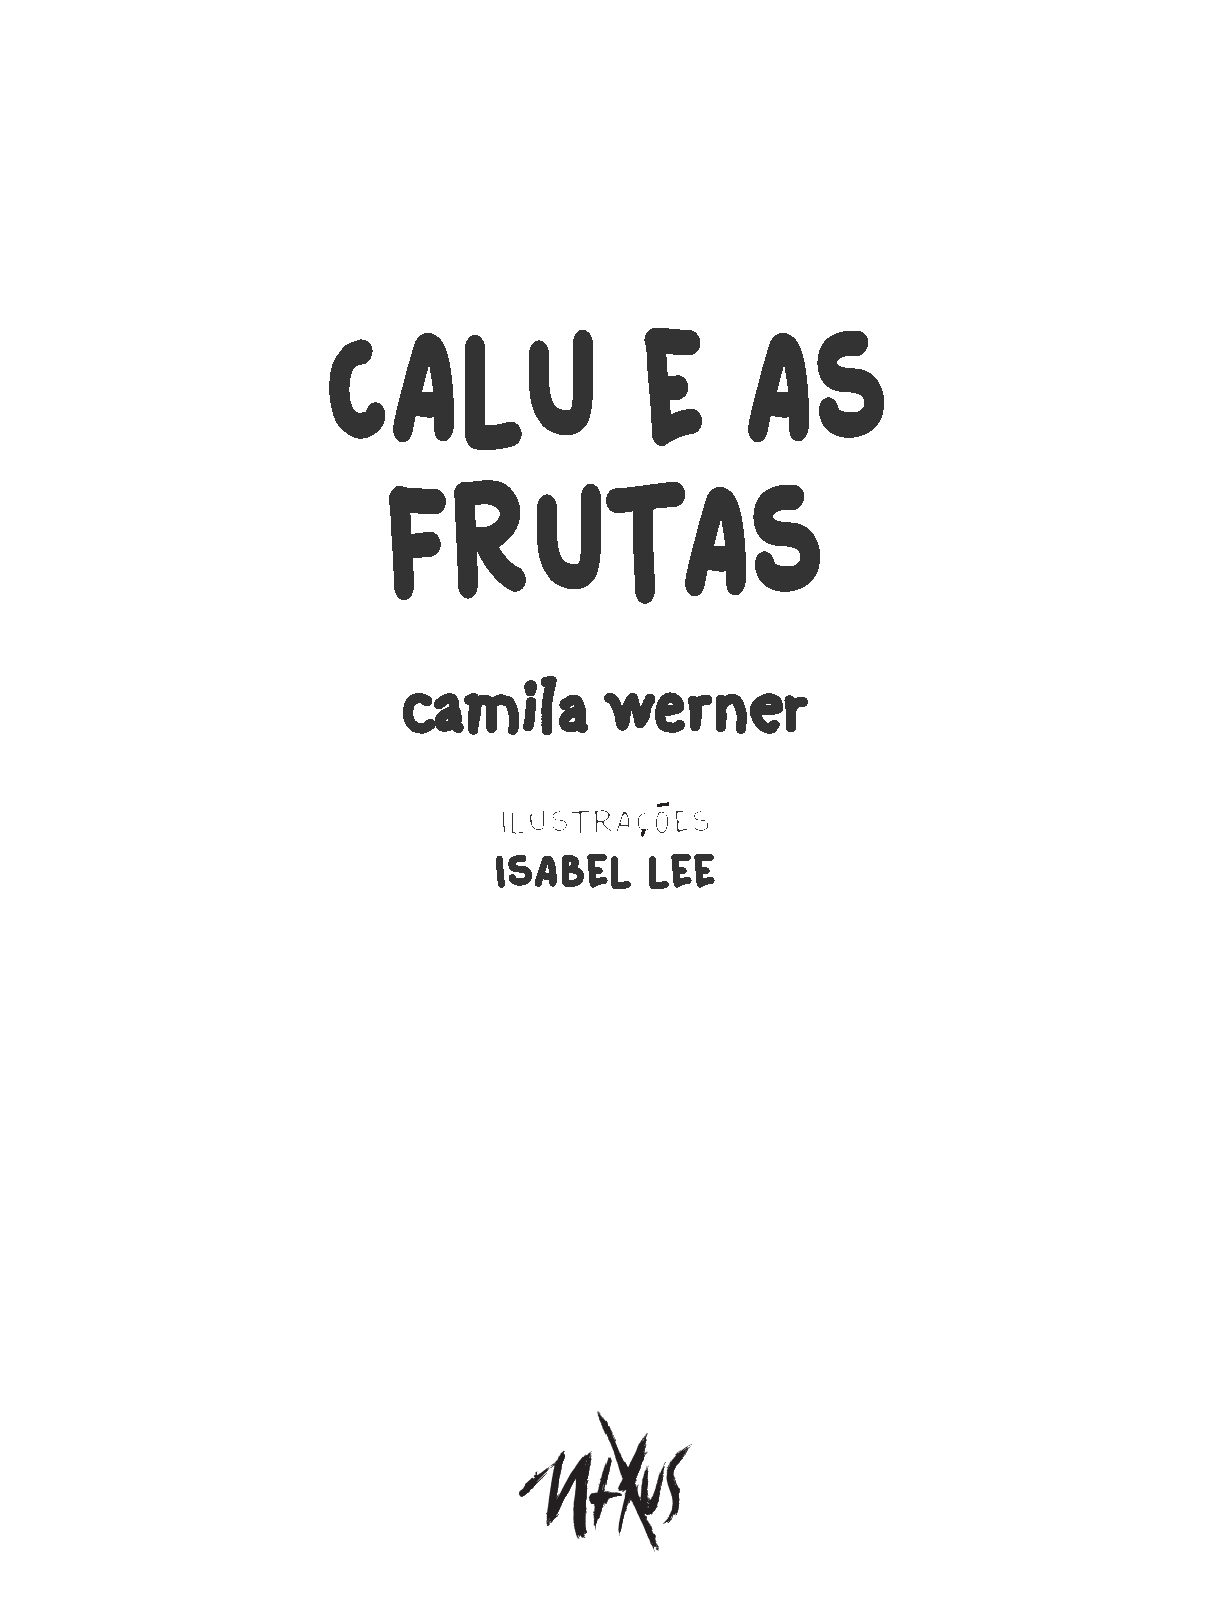
\includepdf[nup=2x2, 					% grid
			% offset=-15mm -5mm, 		% posição
			% scale=.8, 				% tamanho da página
            % delta=4mm 4mm, 			
            % frame,
            % pages={1-4}]{pdfs/PNLD2022-018_MIOLO.pdf}

\end{document}
